%%%%%%%%%%%%%%%%%%%%%%%%%%%%%%%%%%%%%%%%%%%%%%%%%%%%%%%%%%%%%%%%%%%%%%%%%%%%%%%%%%%%%%%%%%%%%
%%									section.	Approches de partitionnement										%
%%%%%%%%%%%%%%%%%%%%%%%%%%%%%%%%%%%%%%%%%%%%%%%%%%%%%%%%%%%%%%%%%%%%%%%%%%%%%%%%%%%%%%%%%%%%%

\section{Approches de partitionnement de graphes}
 Le partitionnement d'un graphe consiste à trouver une partition des sommets respectant une ou plusieurs propriétés. Ces propriétés sont de nature très diverses. On peut par exemple chercher à minimiser la capacité des arêtes externes, c'est-à-dire le nombre d'arêtes ou la somme totale des poids des arêtes reliant deux groupes.  Le problème devient difficile si on cherche à diviser le graphe en $k$ groupes de tailles équilibrées car il n'existe alors pas d'algorithme polynomial pour y répondre. Ce problème a été démontré NP-complet \citep{HYAFIL1973}, \citep{GAREY1976}

Au cours des dernières années, beaucoup d'efforts ont été consacrés au développement d'heuristiques rapides et efficaces pour ce problème. Ces heuristiques peuvent souvent gérer des graphes assez grands avec des milliers de nœuds et fournir de bonnes solutions. Pour un aperçu plus détaillé, nous nous référons à \citep{BichotSiarry2013}, \citep{BULU2016},\citep{SCHLOEGEL2000}.

Nous allons maintenant présenter les approches couramment utilisées pour résoudre le problème du partitionnement de graphes.


\subsection*{Approche exacte}
Les solutions exactes peuvent être utilisées comme des facteurs importants pour valider les heuristiques. Cependant, peux d'effort ont été faits dans le développement d'algorithmes exacts \citep{Armbruster2008}, \citep{Bonami2012}, \citep{Delling2012}, \citep{FeldmannWidmayer2015}, \citep{Ferreira1998}, \citep{Hager2013}, \citep{Kaibel2011}, \citep{Sellmann2003}, \citep{Sorensen2007}. La plupart de ces méthodes reposent sur la méthode de séparation et d'évaluation qui permet d'éviter l'exploration systématique de l'espace des solutions en éliminant les sous-arbres menant à des solutions moins bonnes qu'une solution donnée, et se diffèrent selon que l'exploration de l'arbre est réalisée en profondeur, par niveaux ou par ordre croissant des valeurs des fils non encore traités \citep{Land2010}.
Du fait de la nature NP-difficile du problème, il est clair que généralement seuls des graphes relativement petits peuvent être résolus par une approche exacte.

\subsection*{Approche spectrale}
L'approche spectrale du partitionnement de graphes repose sur le théorème spectral de l'algèbre linéaire, elle consiste à rechercher les valeurs propres de la matrice de Laplace associée au graphe $G$, ensuite l'ordonnancement de ces valeurs qui est lié à la connectivité des sommets du graphe.
Les techniques spectrales ont d'abord été utilisées par Donath et Hoffman \citep{DonathHoffman1972} et Fiedler \citep{Fiedler1973}, \citep{Fiedler1975}, et ont été améliorées par la suite par plusieurs chercheurs \citep{Boppana1987}, \citep{HendricksonLeland1995a}, \citep{Kabelikova2006}, \citep{Simon1991}.
Il a été montré que cette méthode permet d'obtenir un extremum global avec certains graphes \citep{Pothen1990}; cependant, il a aussi été mis en évidence que cette méthode est très coûteuse en terme de calculs et devient inefficaces lorsque la taille du graphe devient importante \citep{BarnardSimon1994}.

\subsection*{L'approche combinatoire} \citep{BENSETIRA2017}
Contrairement à l'approche spectrale, les travaux cités dans cette approche opèrent directement sur la structure du graphe.
L'idée générale consiste à effectuer un parcours de proche en proche d'une partie de l'ensemble $P(G)$ afin d'y trouver le meilleur candidat qui résolve le problème. En plus, un algorithme de ce type nécessite les deux données suivantes :
\begin{itemize}
\item la définition d'un voisinage dans $P(G)$;
\item l'historique des optimisations précédentes.
\end{itemize}
Le voisinage permet de définir comment l'algorithme va progresser en perturbant la solution courante $S$ : par exemple, on peut définir le voisinage de $S$ comme correspondant à un seul déplacement de sommet par l'ensemble des éléments de $P(G)$ qui peuvent être obtenus en changeant dans la partie un seul sommet de $S$.

Dans cette approche, on distingue entre les méthodes basées sur les algorithmes itératifs et les méthodes basées sur les méta-heuristiques.

\subsection*{Les algorithmes itératifs}
Les algorithmes itératifs d'optimisation fonctionnent en partant d'une partition $\prod _0 \;\in \; P(G)$ de $G$, valide et bien équilibrée, et se déplacent dans l'espace des solutions en sélectionnant le voisin le plus proche qui permet de réduire la coupe de la partition. L'algorithme s'arrête lorsqu'aucun des voisins n'est satisfaisant. Ces algorithmes convergent donc vers l'optimum local accessible depuis la partition initiale $\prod _0$ .

Bien que la convergence ne soit que locale et dépendante du point de départ dans $P(G)$, ces algorithmes sont très populaires. Les résultats produits pouvant être améliorés en effectuant plusieurs exécutions à partir de partitions initiales différentes ou en utilisant le schéma multi-niveaux qui sera présenté plus loin. Parmi les algorithmes de cette catégorie, nous pouvons citer \citep{FiducciaMattheyses1988}, \citep{Hagen1997}, \citep{KernighanLin1970}, \citep{Krishnamurthy1984}. 

Le principal défaut de ces approches itératives concerne leur vision strictement locale du problème, ce qui implique que le résultat ne peut être au mieux qu'un optimum local, fortement dépendant de la solution initiale. D'autres approches d'algorithmes d'optimisation ayant une vision plus globale peuvent être utilisées.

\subsection*{Les approches basées sur les méta-heuristiques}
 Les algorithmes génétiques, ont fait l'objet de plusieurs approches pour le problème du partitionnement de graphes \citep{BuiMoon1996}, \citep{ChevalierPellegrini2006}, \citep{ChockalingamArunkumar1992}, \citep{Soper2004}, \citep{TalbiBessiere1991}.  Le principe est d'explorer l’espace des solutions à l'aide d'une population d'individus qui vont échanger entre eux certaines de leurs caractéristiques lors d'une étape de reproduction, ceci dans le but d'obtenir de nouveaux individus combinant les qualités de leurs parents tout en essayant d'en diminuer les défauts. Pour un aperçu général des algorithmes génétiques abordant le problème du partitionnement de graphe, nous renvoyons le lecteur à l'article de \citep{Kim2011}.

Les principales difficultés d'application de ces algorithmes tiennent d'une part à la multitude de paramètres qu'il faut régler en fonction de la nature du problème, d'autre part à leurs coûts en mémoire et en temps : La taille de la population est liée à celle du problème et le temps est dépendant du nombre de générations qui est lié à la taille de la population.

Les méthodes de colonies de fourmis consistent à imiter le comportement des fourmis qui exploitent une méthode de résolution collective. En effet, les fourmis utilisent des phéromones pour marquer les différents chemins empruntés et la concentration de ces marqueurs chimiques est
d'autant plus importante que la fréquence d'utilisation est importante. Pour le k-partitionnement, l'idée est donc d'utiliser $k$ colonies de fourmis dont le but est d'accumuler la nourriture qui est distribuée sur les sommets du graphe, l'exploration est guidée par la répartition des colonies, de la nourriture et par les décisions des fourmis \citep{Korosec2004}, \citep{LanghamGrant1999}, \citep{Jovanovic2016}.

D'autres méta-heuristiques, comme la recherche tabou \citep{BattitiBertossi1999}, le recuit simulé \citep{Bichot2004}, \citep{Johnson1989}, \citep{Williams1991}, les algorithmes de gradients aléatoires adaptatifs (GRASP) \citep{AreibiYang2004}, les méthodes de diffusion stochastique \citep{TaoZhao1993}, \citep{Wan2005}, ont été appliquées avec plus ou moins de succès au partitionnement de graphe.

On peut aussi citer les travaux basés sur la méthode de percolation \citep{MeyerhenkeSchamberger2006}, \citep{Pellegrini2007} qui s'inspire du principe de l'écoulement d'un fluide à travers un solide poreux, et la méthode de fusion-fission \citep{Bichot2007} qui s'inspire de la physique nucléaire et plus particulièrement des fusions et fissions d'atomes.
L'efficacité des méthodes combinatoires est étroitement liée à la taille de l'espace de recherche, les heuristiques calculent un partitionnement acceptable en un temps polynomial.


\subsection*{L'approche multi-niveaux}
La méthode multi-niveaux, introduite par \citep{BarnardSimon1994}, \citep{HendricksonLeland1995b}, \citep{VanDriesscheRoose1994}, permet de réduire la taille du graphe ainsi que celle de l'espace de recherche tout en procurant l'accès à une vision globale pour les algorithmes
combinatoires. L'idée principale est de travailler sur un graphe réduit ayant les mêmes propriétés topologiques que le graphe initial (regrouper les sommets ensemble pour traiter de groupes de sommets plutôt que de sommets indépendants).
Pour ce faire, le schéma multi-niveaux comporte trois étapes (Figure \ref{pmn}) :
\begin{enumerate}
	\item  L'étape de contraction, durant laquelle on applique récursivement une fonction de contraction afin de diminuer la taille du graphe;
	\item  L'étape de partitionnement initial, où l'on applique une heuristique sur le plus petit graphe;
	\item  L'étape d'affinage, durant laquelle la partition initiale est projetée et raffinée sur les graphes de plus en plus gros jusqu'au graphe initial.
\end{enumerate}
  
	\begin{center}
		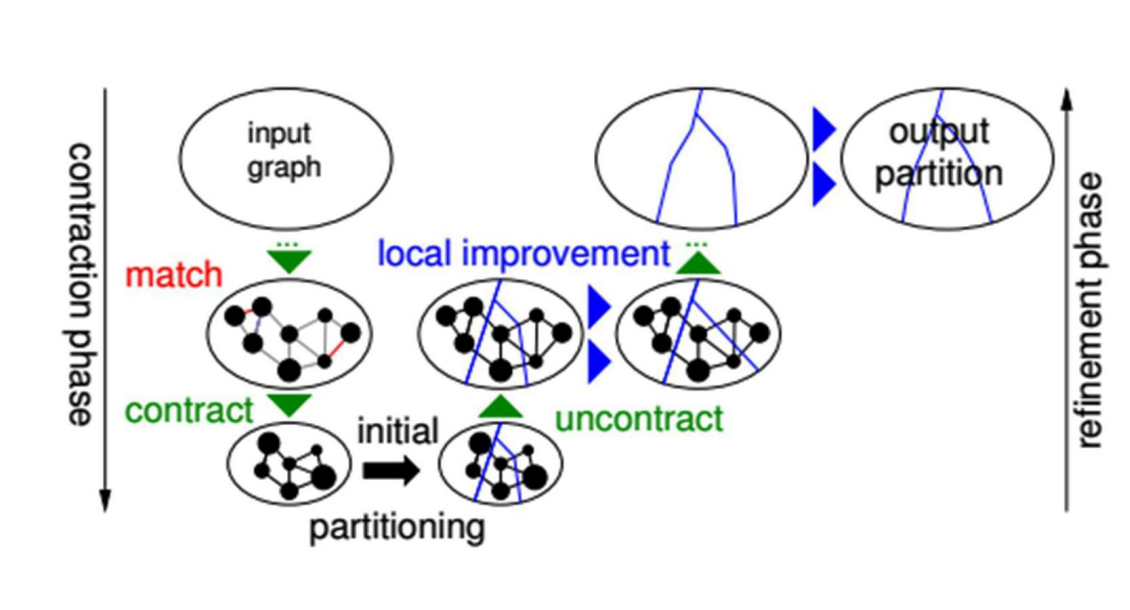
\includegraphics[height=2in]{img/multiniveaupartitionnement.PNG}		
		\captionof{figure}{ L'approche multi-niveau du partitionnement de graphe, \citep{SandersSchulz2011}} \label{pmn}
	\end{center}
Dés lors, plusieurs améliorations ont été proposées \citep{Aurora2007}, \citep{ChevalierSafro2009}, \citep{KalayciBattiti2018}, \citep{Karypis2003}, \citep{KarypisKumar1998}, \citep{Monien2000}, \citep{Pellegrini1995}, \citep{Pope2016}, \citep{Predari2017}, \citep{Safro2015}, \citep{SandersSchulz2011}, \citep{Talu2017}.


\subsection*{La parallélisation du partitionnement de graphes}
Des tentatives de parallélisation des algorithmes de partitionnement de graphes ont vu le jour. On peut citer ParMeTiS \citep{Karypis2011}, ParJostle \citep{Walshaw2012}, PT-Scotch \citep{ChevalierPellegrini2008}, et Parkway \citep{TrifunovicKnottenbelt2004} pour le partitionnement d'hyper-graphes. Tous ces outils utilisent un schéma multi-niveaux parallèle.

Des approches qui combinent les différentes méthodes présentées ci dessus ont été proposées, \citep{Chan2016}, \citep{LaSalleKarypis2013}, \citep{LaSalleKarypis2015}, \citep{LengYu2007}, \citep{Rahimian2013}, \citep{SandersSchulz2012}, \citep{Tashkova2011}.


